
%\vspace{-3mm}

\section{Experimental Setup}
%In this section we evaluate the effectiveness of our algorithm as compared to the existing methods. We start by explaining the datasets and baseline sampling algorithms. Then we provide the criteria to evaluate the competing algorithms, followed by a detailed comparative analysis. 
In this section, we describe the baseline sampling algorithms and the datasets used in our experiments.

\subsection{Sampling algorithms}
We compare our method with five existing sampling methods: (i) Streaming Node (SN) \cite{ahmed2014network}, (ii) Streaming Edge (SE) \cite{ahmed2014network}, (iii) Streaming BFS (SBFS) \cite{ahmed2014network}, (iv) PIES \cite{ahmed2010reconsidering}, and (v) Green algorithm (GA) \cite{tong2016novel}. The first four algorithms are exclusively designed for streaming graphs while the last one is designed for static graphs. Note that unlike ours, none of the existing algorithms explicitly produce a community structure as a bi-product of the sampling\footnote{Although GA claims that its sample graph preserves the underlying community structure, it does not explicitly produce the community structure.}, and thus one needs to execute community detection algorithm separately on the sample to obtain the community structure. Therefore to evaluate the competing algorithms with respect to how the underlying community structure in the sample resembles with that of the original graph, for SN, SE, SBFS and PIES we run Louvain algorithm~\cite{blondel2008fast} on each individual sample and detect the communities. In case of GA, we consider the aggregated graph and run GA to obtain the sample, and further run Louvain on the sample to detect the community structure. Note that although by considering the aggregated graph GA acquires far more information of the entire graph structure, we use it as a strict baseline in this study to show that the community structure obtained from \compas~is quite competitive to that obtained by running Louvain on GA's sample graph.   






\subsection{Datasets}\label{sec:dataset}

We perform our experiments on five graphs mentioned below. While first two are streaming graphs, last three graphs are static graphs. \\
(i) {\bf Facebook}\footnote{konect.uni-koblenz.de/networks/facebook-wosn-links}:
  	This is an undirected graph with  nodes representing users, and an edge exists between two users if they are friends. Each edge is time stamped by the occurrence of the friendship. 
    The graph consists of $63,731$ nodes and $817,035$ edges.\\ % \TODO{Is there a ground truth community structure? Else how do you obtain communities here?} \textcolor{blue}{done}\\
 (ii) {\bf arxiv hep-th}\footnote{konect.uni-koblenz.de/networks/ca-cit-HepTh}:
    This dataset represents the collaboration graph of the authors in arXiv's High Energy Physics papers. Each node represents an author and an edge exists between two authors if they have co-authored a paper. The edges are time stamped by publication date of the co-authored paper. The graph consists of 22,908 nodes and 2,673,133 edges.\\% \TODO{Is there a ground truth community structure? Else how do you obtain communities here?}\textcolor{blue}{done}\\ 
(iii) {\bf Youtube}\footnote{snap.stanford.edu/data/com-Youtube.html}:
This dataset represents the Youtube social network with nodes representing users and edges representing friendship. The graph consists of 1,134,890 nodes and 2,987,624 edges. \\
%User created groups in the network form the ground truth community structure. There are 8,385 communities in the ground truth.\\
(iv) {\bf Dblp}\footnote{snap.stanford.edu/data/com-DBLP.html}:
This dataset consists of authors indexed in DBLP. The graph is same as arxiv hep-th. There are 317,080 nodes and 1,049,866 edges in the graph. \\
%Publication venue defines ground truth communities. There are 13,477 communities in the ground truth.\\
(v) {\bf LFR}: This is a synthetic graph 
 \cite{lancichinetti2008benchmark} with underlying community structure implanted into it. We construct the graph with  25,000 nodes, 254,402 edges and 18,34 communities.


%The first three datasets were presented by Yang et.~al. in \cite{yang2015defining}.
%Although the above graphs are all static, we assign 
Since last three graphs are static, we consider that each edge arrives in a pre-decided order (which is set randomly) i.e., each edge has a (discrete) time of arrival. We later show that edge ordering does not influence the inferences drawn from the results (Section~\ref{sec:effect}).

Moreover, since first four graphs do not have any underlying ground-truth community structure, we run Louvain algorithm \cite{blondel2008fast} on the aggregated graph and obtain the disjoint community structure. This community structure is the best possible output that we can expect from our incremental modularity maximization method, and therefore serves as the ground-truth. 

%\vspace{-3mm}
\section{Evaluation}
We design a two-fold experimental setup. First, we show how  competing sampling algorithms detect the original community structure, and second, we measure how good individual samples are w.r.t. the structural properties of the original graph. Although the primary focus of \compas~is to quality better in the first evaluation, we also show that \compas~is quite competitive to retain the graph structure in the second evaluation.


\begin{table*}[!t]
\centering
\caption{\label{tab_all}Summary of the $D$-statistics (the lower, the better) values of the topological measures for all the datasets. For Youtube we present all the results, while for the rest we provide the average $D$-statistics and standard deviation (SD). \compas~truns out to the second best algorithm after GA (the most informed static graph sampling algorithm for which the sample is obtained from the aggregated graph and Louvain is run on the sample, thus serving as the strict baseline). Top two values for each average result is highlighted.}% \TODO{Provide standard deviation/error $\sigma$ for the last 4 networks.}}


\begin{adjustbox}{max width=\textwidth}
\begin{tabular}{l|c c c c c c c c c c c c c |c |c|c|c|c}
\hline
 \multirow{2}{*}{Algorithm}          & \multicolumn{14}{c|}{Youtube}                                                       & Facebook  & Com-dblp & LFR & hep-th    \\ \cline{2-19}
 & ID & EI & AD & FOMD & TPR & EX & CR & CON & NC & AODF & MODF & FODF & MOD & Avg,SD & Avg,SD & Avg,SD  & Avg,SD & Avg,SD \\ \hline
\compas     & 0.063   & 0.051   & 0.078    & 0.057     & 0.227    & 0.082   & 0.054   & 0.091    & 0.260   & 0.073    & 0.201     &  0.121    & 0.052    & {\bf 0.10,0.07}   & {\bf 0.17,0.09}  &  {\bf 0.16,0.10}   & {\bf 0.18,0.06} &  {\bf 0.10,0.03 }   \\ 
SN         & 0.164   &  0.171  & 0.471   & 0.061     & 0.542    & 0.581   & 0.112   & 0.265    & 0.064   & 0.157     & 0.182     & 0.092     &  0.216   &  0.23,0.17  &       0.33,0.17  &    0.29,0.20      &  0.27,0.07 &  0.26,0.04    \\ 
SE         &  0.257  & 0.244   & 0.241   & 0.501     & 0.281    & 0.098   & 0.287   & 0.087    & 0.151   & 0.097     &  0.246    &  0.093    & 0.198    &  0.21,0.11  &       0.27,0.11  &   0.25,0.14       &   0.32,0.08  & 0.29,0.06   \\ 
SBFS       &  0.126  & 0.131   & 0.172   &  0.106    & 0.454    & 0.145   & 0.056   & 0.165    & 0.045   &   0.257   & 0.108     & 0.076     & 0.181    &  0.15,0.10  &        0.26,0.09  &  0.24,0.10        &  0.25,0.09 &  0.26,0.04    \\ 
PIES       &  0.234  & 0.241   &  0.252  & 0.190    & 0.409    & 0.042   & 0.051   & 0.049    & 0.061   &      0.157 & 0.042     & 0.053     & 0.121    &  0.14,0.10  &         0.29,0.06  &   0.24,0.07       &  0.26.0.05  &  0.21,0.05   \\ 
GA         &   0.156 & 0.055   & 0.065   & 0.053     & 0.267    & 0.066   & 0.076   & 0.053    & 0.085   &   0.150   & 0.075     &  0.069    & 0.102    &  {\bf 0.09,0.06} & {\bf 0.12,0.04}   &   {\bf 0.12,0.06}  &  {\bf 0.14,0.06} &  {\bf 0.08,0.04}    \\ \hline
\end{tabular}
\end{adjustbox}
%\vspace{-5mm}
\end{table*}



\subsection{Community-centric evaluation}
In this section, we start by explaining the metrics used to evaluate the goodness of the community structure, followed by a detailed comparison of the sampling algorithms.
\subsubsection{Evaluation criteria}
To measure how sampling algorithms capture the underlying community structure, we evaluate them in two ways.  First we measure the quality of the obtained community structure based on the {\bf topological measures} defined by Yang et.~al.  \cite{yang2015defining}. In particular, we look into four classes of quality scores - (i) {\em based on internal connectivity}: internal density (ID), edge inside (EI), average degree (AD), fraction over mean degree (FOMD), triangle participation ratio (TPR); (ii) {\em based on external connectivity}: expansion (EX), cut ratio (CR); (iii) {\em combination of internal and external connectivity}: conductance (CON), normalized cut (NC), maximum out-degree fraction (MODF), average out-degree fraction (AODF), flake out-degree fraction (FODF); and (iv) {\em based on graph model}: modularity (MOD)\footnote{See \cite{yang2015defining} for the detailed definitions of all these metrics.}. Note for every individual community we obtain a score, and therefore a distribution of scores (i.e., distribution of ID, distribution of EI etc.) is obtained for all the communities of a graph. We measure how similar (in terms of Kolgomorov-Smirnov $D$-statistics\footnote{It is defined as $D = max_x\{|f(x) - f^{'}(x)|\}$ where $x$ is over the range of the random variable, and $f$ and $f^{'}$ are the two empirical cumulative distribution functions of the data.}) these distributions are with those of the ground-truth communities. {\em The less the value of D-statistics, the better the match between two distributions}.

%We further measure the community quality based on the ground-truth community structure. Finally, we calculate the Kolgomorov-Smirnov $D$-statistics between the community score distribution obtained from the sample and the ground truth for each individual type of score. Note that $D$-statistics is applied as a part of Komogorov-Smirnov test to reject the null hypothesis. Here we use it to measure the agreement between the two distributions. 


As a second level of evaluation,  we use the {\bf community validation metrics} --  Purity~\cite{manning2008introduction}, Normalized Mutual Information (NMI)~\cite{danon2005comparing} and Adjusted Rand Index (ARI)~\cite{hubert1985comparing} to measure the similarity between the ground-truth and the obtained community structures. {\em The more the value of these metrics, the more the similarity.}

\if{0}
\begin{table*}[!t]
\centering
\caption{\label{g_metric_alg}Purity (PU), NMI and ARI values between the ground-truth and community structure obtained from individual sampling algorithms for all datasets.}
\scalebox{0.7}{
\begin{tabular}{l |>{\columncolor[gray]{0.8}} c>{\columncolor[gray]{0.8}}  c>{\columncolor[gray]{0.8}}  c|  c  c  c| ccc|ccc|ccc|>{\columncolor[gray]{0.8}}c>{\columncolor[gray]{0.8}}c>{\columncolor[gray]{0.8}}c}
\hline
\multirow{2}{*}{{\bf Dataset}} & \multicolumn{3}{c|}{{\bf \compas}} & \multicolumn{3}{c|}{{\bf SN}} & \multicolumn{3}{c|}{{\bf SE}} & \multicolumn{3}{c|}{{\bf SBFS}} & \multicolumn{3}{c|}{{\bf PIES}} & \multicolumn{3}{c}{{\bf GA}} \\\cline{2-19}
   & \multicolumn{1}{c}{PU} & \multicolumn{1}{c}{NMI} & \multicolumn{1}{c|}{ARI} & PU & NMI & ARI &PU & NMI & ARI &PU & NMI & ARI &PU & NMI & ARI & \multicolumn{1}{c}{PU} & \multicolumn{1}{c}{NMI} & \multicolumn{1}{c}{ARI} \\\hline
Facebook	  & 0.71 & 0.52 & 0.47	 & 0.43&0.34&0.26  & 0.39&0.28&0.12  &  0.53&0.41&0.18  & 0.57&0.48&0.36  & 0.76&0.61&0.52 \\
hep-th		  &	0.69&0.51&0.38 & 0.39&0.32&0.19 & 0.29&0.21&0.12 & 0.42&0.36&0.25  & 0.48&0.39&0.31 & 0.74&0.68&0.57\\
youtube		      & 0.83&0.72&0.67	 &  0.52&0.49&0.36 & 0.48&0.33&0.28  &  0.63&0.58&0.47 & 0.56&0.51&0.41  & 0.86&0.77&0.71 \\
Dblp		  &	0.72&0.65&0.58 & 0.32&0.28&0.21  & 0.29&0.21&0.16  & 0.66&0.57&0.32  & 0.48&0.39&0.31  & 0.79&0.69&0.52 \\
LFR		  & 0.76&0.69&0.55	 & 0.35&0.29&0.21  & 0.56&0.32&0.29  & 0.49&0.38&0.26  & 0.42&0.31&0.28  &  0.81&0.72&0.67 \\\hline
Average & 0.74 & 0.61 & 0.53 & 0.40 & 0.34 & 0.24 & 0.40 & 0.27 &0.19 & 0.54 & 0.46 & 0.29 & 0.50 & 0.41 & 0.33 & 0.79 & 0.69 & 0.59   \\
\hline
\end{tabular}}

\end{table*}
\fi


%\vspace{-3mm}
\subsubsection{Parameter estimation}

As reported in Section \ref{algorithm}, our algorithm consists of two parameters (i) $\alpha$ (initial fraction of nodes inserted), (ii) $n_d$ (length of the buffer).
%In Figures \ref{param_est}(a) and \ref{param_est}(b) we plot the average  $D$-statistics for different values of $\alpha$ and $n_d$ respectively. 
For $\alpha$, we observe that D-statistics is initially high and reduces as we increase $\alpha$ (Figures \ref{param_est}(a)). This is because for low $\alpha$ values the community structure obtained initially by running Louvain algorithm (Step 12 in Algorithm 1) is coarse. For large values of $\alpha$ even though initial community structure obtained is good, it is not allowed to evolve much. Similarly in Figure~\ref{param_est}(b), given a small buffer size several nodes mostly arriving once would be added to the sample leading to formation of pendant vertices. As we increase the buffer size \compas~performs better till a certain point, after which the improvement is negligible. Since we are interested in using minimum space we fix $n_d$ at $0.001\cdot n$. 
Thus, for the rest of the experiments we set $\alpha$ to $0.5$ and $n_d$ to $0.001\cdot n$ unless otherwise specified. Further we set $n$ to $0.4|V|$ as default (see Section \ref{sec:effect} for different values of $n$).

%\vspace{-2mm}
\begin{figure}[!h]
\centering
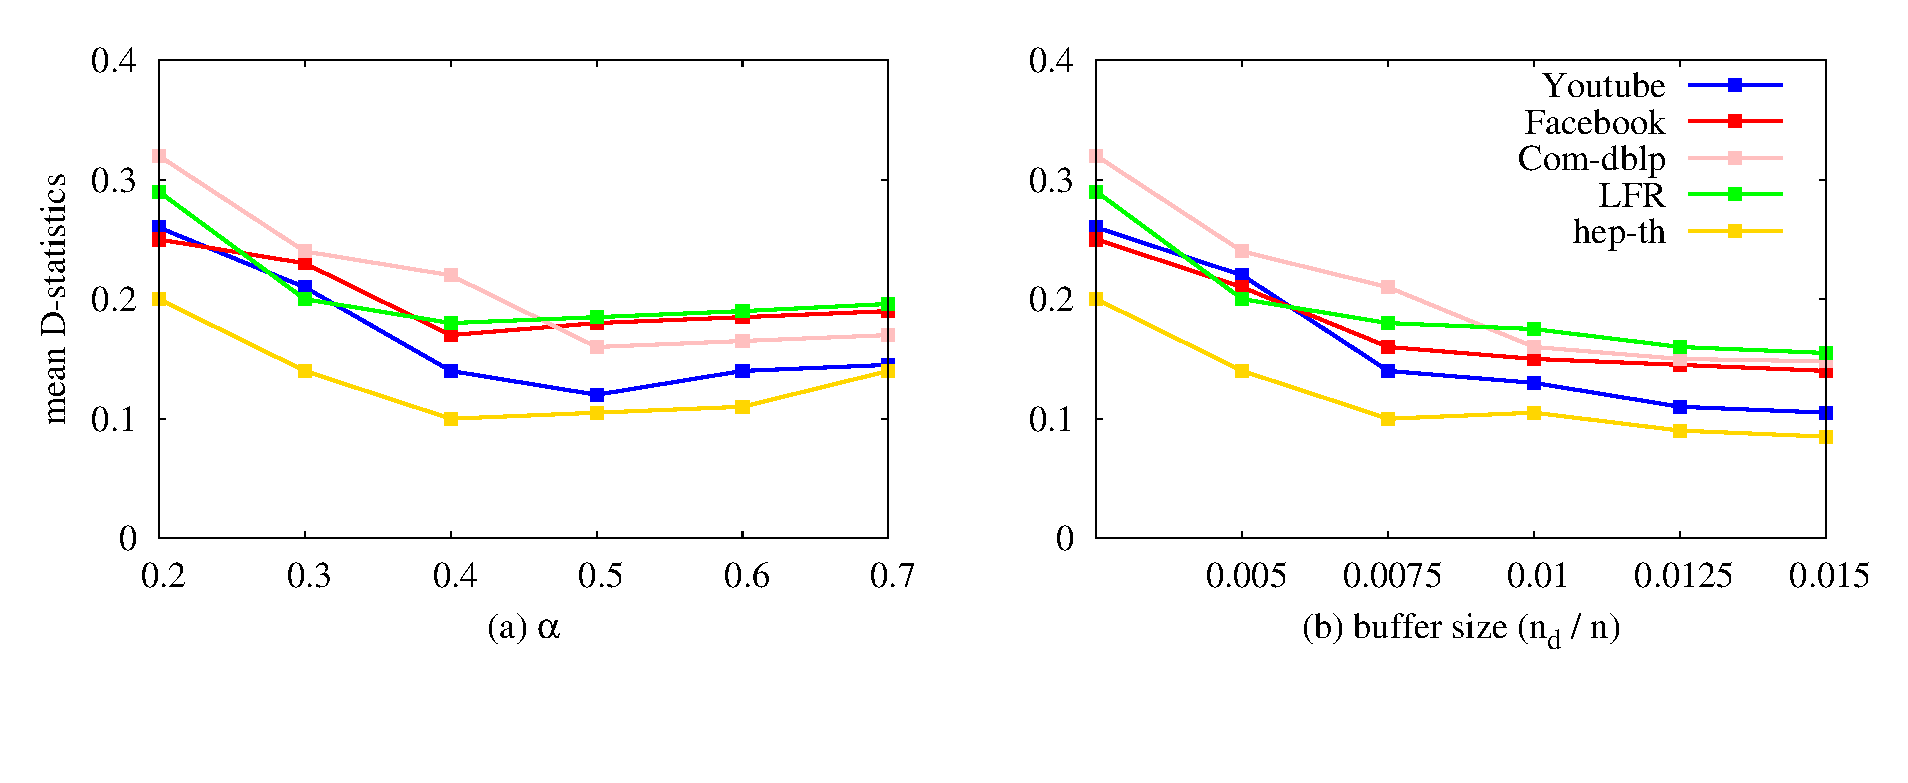
\includegraphics[scale=0.4]{./texfiles/Chapter_2/figures/param_estimate.eps}
%\vspace{-12mm}
\caption{\label{param_est}Average $D$-statistics value across all the topological measures.}
%\vspace{-5mm}
\end{figure}



\begin{table}[!t]
\centering
\caption{\label{g_metric_alg}NMI between the ground-truth and community structure obtained from individual sampling algorithms for all datasets.}
\scalebox{0.7}{
\begin{tabular}{l cccccc}
\hline
\multirow{1}{*}{{\bf Dataset}} & \multicolumn{1}{c}{{\bf \compas}} & \multicolumn{1}{c}{{\bf SN}} & \multicolumn{1}{c}{{\bf SE}} & \multicolumn{1}{c}{{\bf SBFS}} & \multicolumn{1}{c}{{\bf PIES}} & \multicolumn{1}{c}{{\bf GA}} \\\hline
Facebook	  & 0.52 & 0.34 & 0.28&0.41&0.48&0.61\\
hep-th		  &0.51&0.32&0.21&0.36&0.39&0.68\\
Youtube		      &0.72&0.49&0.33&0.58&0.51&0.77 \\
Dblp		  &0.65&0.28&0.21&0.57&0.39&0.69 \\
LFR		  &0.69&0.29&0.32&0.38&0.31&0.72\\\hline
Average & {\bf 0.61}  & 0.34 & 0.27 & 0.46  & 0.41 & {\bf 0.69}    \\
\hline
\end{tabular}}
%\vspace{-5mm}
\end{table}

\subsubsection{Comparison of sampling algorithms}

We start by measuring the similarity between the obtained and the ground-truth community structures using topological measures. In Table~\ref{tab_all} we summarize the $D$-statistics values of all the scoring functions for Youtube dataset; for the other graphs we only present the average value (and standard deviation) across the $D$-statistics among different topological measures (see \cite{si} for detailed results). \iffalse\TODO{For these networks we MUST report standard deviation/error}.\fi Clearly~\compas~outperforms all the streaming algorithms across different datasets. GA performs better than~\compas~since it has in its consideration the whole graph to obtain the sample. However, we stress that even with {\em minimal community information to start with} and {\em no subsequent community detection in the later steps}, we are able to reach very close to GA as well as to the ground-truth.

As a second level of evaluation, we further calculate three validation metrics -- purity, NMI and ARI  between the ground-truth and the obtained community structure for all the algorithms (see Table \ref{g_metric_alg}  for NMI, details in \cite{si}). Once again we observe that \compas~is the second ranked algorithm after GA with an average (over all datasets) purity, NMI and ARI of 0.74, 0.61 and 0.53 respectively.
%which is followed by SBFS, PIES, SN and SE.

\subsection{Graph-centric evaluation}
\label{graph_evaluation}
Although our primary objective is to obtain a community-preserved graph sample, we further evaluate our sample in terms of three graph properties mentioned in \cite{ahmed2014network}: (i) degree distribution (Degree), (ii) clustering coefficient distribution (CC), (iii) top 100 eigen value distribution (EV). 
In Table \ref{graph_prop} we report the $D$-statistics values between the distributions of the original graph and those obtained from the sample (see more results in \cite{si}). For all the datasets, we observe that \compas~stands within top three ranks in terms of low $D$-statistics, in many cases, also beating the strict baseline GA. This essentially indicates that \compas, apart from preserving the community structure, also preserves general graphs properties in the sample.

%\vspace{-2mm}
\begin{table}[!h]
\centering
\caption{Summary of $D$-statistics for different graph properties. For Youtube we present all the results, while for the rest we provide only average $D$-statistics (top three results in each average case are highlighted).}
\label{graph_prop}
\begin{adjustbox}{max width=\columnwidth}
\begin{tabular}{l|c c c |c|c|c|c|c}
\hline
  \multirow{2}{*}{Algorithm}         & \multicolumn{4}{c|}{Youtube}     & Facebook & Com-dblp & LFR     & hep-th  \\ \cline{2-9}
& Degree & CC & EV & Average & Average  & Average  & Average & Avearge \\ \hline
\compas    &   0.083     & 0.105   & 0.42     &  {\bf 0.20}       &  {\bf 0.17}        &  {\bf 0.16}       & {\bf 0.28}        & {\bf 0.18}       \\ 
SN        &    0.076    & 0.108   &  0.54     &  0.24             &   0.36             &  0.24             & 0.34              &  0.23       \\ 
SE        &    0.114    & 0.195   &  0.39     &  0.23             &   0.48             &  0.28             & 0.39              &  0.27       \\ 
SBFS      &    0.105    & 0.172   &  0.32     &  {\bf 0.19}       &   {\bf 0.28}       &  {\bf 0.13}       & {\bf 0.26}        & {\bf 0.19}       \\ 
PIES      &    0.046    &  0.129  &  0.38     &  {\bf 0.18}       &   {\bf 0.16}       &  0.21             & {\bf 0.28}        & {\bf 0.16}        \\ 
GA        &    0.218    &  0.063  &  0.46     &  0.24            &   0.35             &  {\bf 0.12}       & 0.32              &  0.20       \\ \hline
\end{tabular}
\end{adjustbox}
%\vspace{-1mm}
\end{table}

 
\subsection{Effect of edge ordering and sample size}\label{sec:effect}
As mentioned in Section \ref{sec:dataset}, we artificially imposed an edge ordering for two static graphs -- Youtube and LFR. In this section, we show that most of our inferences are valid irrespective of any edge ordering. To do so, we randomly pick one pair of edges and swap their arrival time. We repeat it for 20\% of  edges present in each static graph. The entire experiment is repeated $20$ times and the average value is reported. Figure \ref{param_est_1}(a) shows that for Youtube graph edge ordering does not affect much the final sample obtained (the pattern is same for LFR graph, see \cite{si}). 

%\TODO{Mention how you obtained the ordering each time? Is it different random order or is there some strategic order also. You should make it explicit and say that~\compas~is tolerant to only these orders. DONE} 
%\textcolor{blue}{To obtain arrival sequences we consider two edges and swap their arrival times. This we do for 20\% of the total edges in the original network.}

Lastly, we present the effect of sample size ($n$) on the obtained community structure. We plot average $D$-statistics values across all the topological measures for all the algorithms on Youtube dataset (see others in \cite{si}) as a function of $n$ (Figure \ref{param_est_1}(b)). As expected, with the increase of $n$ we obtain better results. Interestingly, for~\compas~and GA, the pattern remains consistent compared to others.

%\vspace{-3mm}
\begin{figure}[!h]
\centering
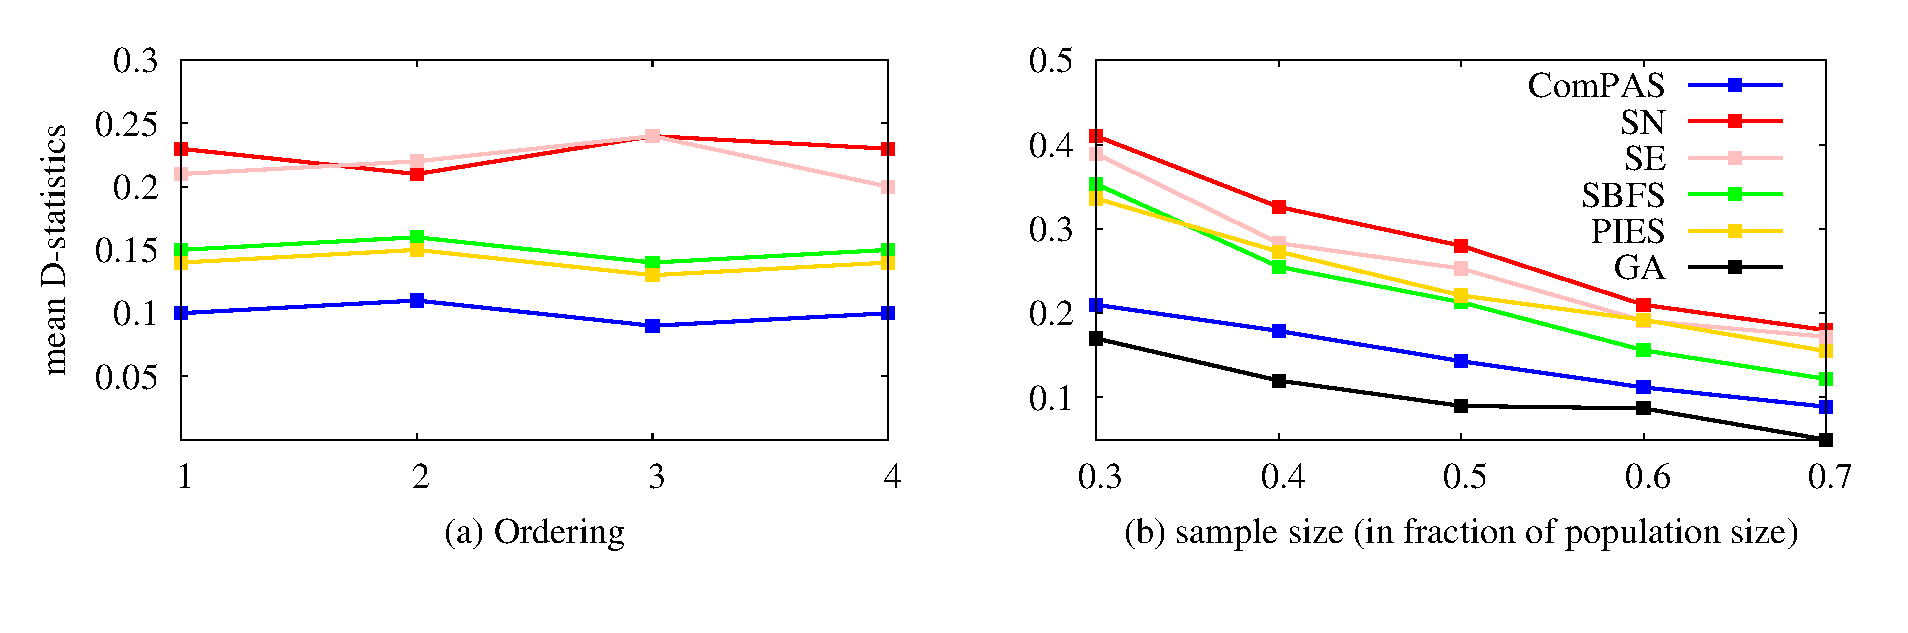
\includegraphics[scale = 0.4]{./texfiles/Chapter_2/figures/param_estimate_1.eps}
%\vspace{-10mm}
\caption{\label{param_est_1}Average $D$-statistics across all the topological measures for (a) different edge ordering and (b) sample size ($n$) of Youtube graph.}
%\vspace{-4mm}
\end{figure}


%\if{0}

%\fi




